\documentclass{beamer}
\usetheme{boadilla}


\usepackage{amsmath,amssymb,amsthm} 
\usepackage{gensymb}
\usepackage{preview}
\usepackage{bm}
\usepackage{mathtools}
\usepackage{hyperref} 
\usepackage{fancyhdr}
\usepackage{indentfirst}
\usepackage{tablefootnote}
%\usepackage{cmbright}
\usepackage[russian, english]{babel}
\usepackage[T1,T2A]{fontenc}
\usepackage[utf8]{inputenc}
\usepackage [autostyle, english = american]{csquotes}
\MakeOuterQuote{"}

\title{Clustering, Mixtures, and the EM Algorithm}
\subtitle{Machine Learning: Module 1}
\author{Sean Norton; Simon Hoellerbauer}
\begin{document}
\begin{frame}
	\titlepage
\end{frame}

\section{Cluster Analysis}

\begin{frame}
\frametitle{The Problem: Finding Groups}
	In social science, we often believe our observations have some sort of group structure.
	\begin{itemize}
		\item Regime types
		\item Types of voters
		\item Types of legislators		
	\end{itemize}
	However, our data doesn't (generally) come with these groupings conveniently pre-labeled.

\end{frame}

\begin{frame}
\frametitle{E.g. Regime Types}
	
	\begin{figure}
		\centering
		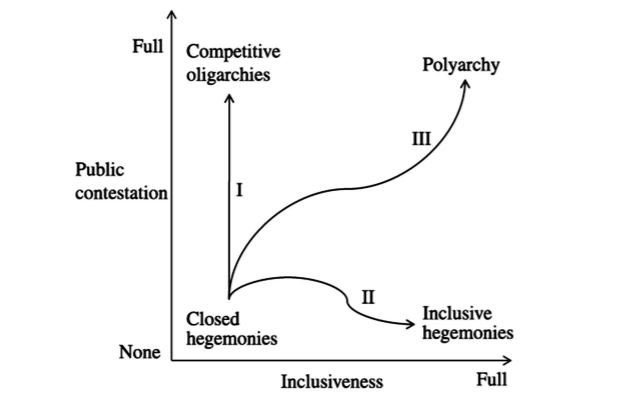
\includegraphics[width=0.7\linewidth]{dahl}
		\caption{Dahl: Regime Types}
		\label{fig:dahl}
	\end{figure}

\end{frame}

\begin{frame}
\frametitle{The Problem Continued}
	The general approach to dealing with this problem has been to hand-label cases. This is problematic because:
	\begin{itemize}
		\item It's time-consuming
		\item Humans aren't able to consider all available data at once
		\item It relies on researcher discretion
		\item For large datasets (e.g. all countries in the world), this is impossible.
	\end{itemize}
	What if there was a way to find latent groupings between our cases quickly and with as little researcher discretion as possible?
\end{frame}

\begin{frame}
\frametitle{Enter Cluster Analysis}
	This is exactly what cluster analysis is intended to do!\\
	Given:
	\begin{itemize}
		\item Data
		\item Number of clusters
		\item Variables
		\item Similarity measure
	\end{itemize}
	A cluster analysis algorithm finds groupings, or clusters, that maximize the similarity between observations within a cluster. 
\end{frame}

\begin{frame}
\frametitle{K-Means and Notation}
	One of the most common similarity measures is the squared distance between the center (mean) of a cluster. \\
	This is known as \textit{k-means} or \textit{k-nearest neighbor} clustering.\\
	Before we dive into the math, some notation:
	\begin{itemize}
		\item $k$: total number of clusters
		\item $r_{nk}$: indicator vector of cluster membership for observation $x_n$
		\item $\mu_k$: the centroid of cluster $k$
	\end{itemize}
\end{frame}

\begin{frame}
\frametitle{K-Means: The Math}
	Cluster analysis relies on a measure of similarity, which in k-means is:
	
	\begin{align*}
	J = \sum_{n=1}^{N}\sum_{k=1}^{K} r_{nk}  \| x_n - \mu_k \|^2
	\end{align*}
	This number $J$ is also known as a \textit{distortion measure}.\\
	What (hopefully) familiar thing does this measure look like?
\end{frame}

\begin{frame}
\frametitle{The Math cont.}
	\textbf{Q}: But how do we choose values of $\mu_k$ given that we don't actually know the cluster assignments?\\
	\textbf{A}: We don't!\\
	We can find $k_m$ through a version of the \textit{expectation-maximization algorithm}:
	\begin{enumerate}
		\item Initialize some random values for $\mu_k$
		\item Minimize $J$ w.r.t. $r_{nk}$; i.e. assign cluster memberships in order to minimize distortion
		\item Using the previous $r_{nk}$, minimize J w.r.t to $\mu_k$; i.e., assign new means that minimize distortion
		\item Repeat until convergence ($J$ does not change, or the change falls below some threshold)
	\end{enumerate}

\end{frame}

\begin{frame}
 \frametitle{The Math: Visualized}
 \begin{figure}
 	\centering
 	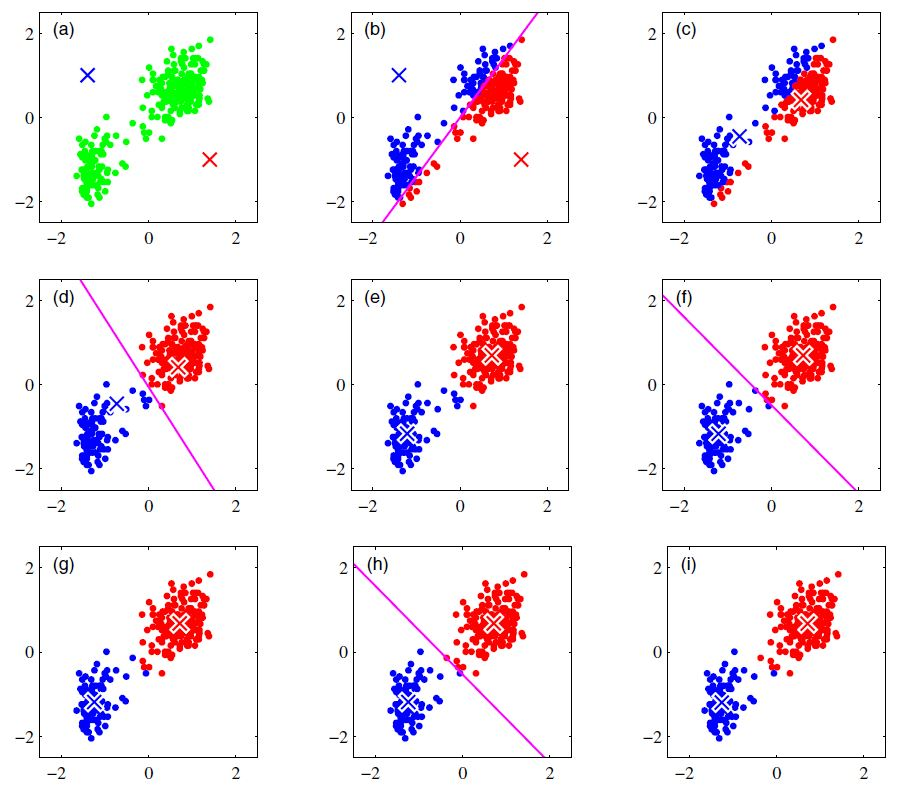
\includegraphics[width=0.7\linewidth]{bishopkmeans}
 	\caption{Optimizing Clusters}
 	\label{fig:bishopkmeans}
 \end{figure}
 
\end{frame}

\begin{frame}
	\frametitle{Problems with Clustering}
	\begin{itemize}
		\item Choosing $k$: this requires trying a lot of different $k$ w.r.t. some similarity measure
			\begin{itemize}
				\item Plot the WCSS against the number of clusters, and look for a "bend" in the plot; this is known as the elbow method
				\item Use average silhouette width: the silhouette is a measure how similar an observation is to its own cluster (consistency) and how dissimilar it is to other clusters (separation)
				\item Gap statistics: compare multiple values of $k$ to a simulated reference distribution of datasets with clusters varying from $k=1$ to $k=max$
			\end{itemize}
		\item Sensitivity to outliers; luckily, there are clustering methods other than $k$-means
			\begin{itemize}
				\item Partitioning around medoids (PAM): uses median instead of mean
				\item Hierarchical clustering: creates a tree-based representation of the data without specifying $k$; clusters are created by "cutting" the tree.  
			\end{itemize}
		\item Fundamentally descriptive; clusters will not necessarily be the same given different data
	\end{itemize}
\end{frame}

\begin{frame}
\frametitle{Problems cont.}



\end{frame}
 

\end{document}
